%\documentclass{beamer}
%\usetheme{Pittsburgh} 
\documentclass{scrartcl}

\usepackage[utf8]{inputenc}
\usepackage{default}
\usepackage[procnames]{listings}
\usepackage{graphicx}
%\usepackage[toc,page]{appendix}
\usepackage{caption}
\usepackage{hyperref}
\usepackage{color}
\usepackage[T1]{fontenc}

%Python
\definecolor{keywords}{RGB}{255,0,90}
\definecolor{comments}{RGB}{0,0,113}
\definecolor{red}{RGB}{160,0,0}
\definecolor{green}{RGB}{0,150,0}
\lstset{language=Python,
basicstyle=\ttfamily\scriptsize,
keywordstyle=\color{keywords},
commentstyle=\color{comments},
stringstyle=\color{red},
identifierstyle=\color{green},
procnamekeys={def,class},
breaklines=true,
columns=fullflexible,
%Numbering and Tabs
%numbers=left,
%tabsize=4,
%showspaces=false,
%showstringspaces=false
}


%Bibliogrpahy?
%\usepackage{bibentry}
%\nobibliography*
%\bibentry{ }


\begin{document}

\title{Evolutionary Computation Theory and Application}
\subtitle{Report}
\author{
  Quignon, Christophe \\
  \href{https://github.com/ChrisQuignon/ECTA}{github.com/ChrisQuignon/ECTA}
  %Familyname, Name
} 
\date{\today}


\maketitle


\setcounter{tocdepth}{2}
\setcounter{secnumdepth}{2}
\tableofcontents{}


\section{Optimization}
%Theoretic description
The first exercise was about the performance of different optimization algorithms on landscapes with raising complexities. The algorithms where simple and had little tuning parameters. They function similar to genetic algorithms by iteratively improving their performance. But they do not run in populations, there is no random mutation and no crossover. 

\subsection{Problem}
\subsubsection{Square error}
The square error function has only one optimum and is among the most simple optimization problems. Only a a very bad parameter choice could lead to not finding an optimum.

\subsubsection{Trimodal fitness function}
The trimodal fitness function has two local optimum and a global optimum in between them. It is simple but can be used to illustrate the problem of overcoming local optima.

\subsubsection{3D plateau fitness function}
The 3D plateau fitness function is more complex then the functions before. It stretched 3 dimensions and not only 2 and has plateaus which are also tricky to overcome. This complexity already ruled out the newton method, because the derivative in 3D is tricky to implement.
%characteristics of the problem

\subsection{Algorithms}
%How do we solve it
\subsection{Hillclimber}
The Hillclimber method is an effective an easy way to find a local optimum by iterative evaluation of all neighbouring points and choosing the best of those. It can be optimised by evaluating more neighbours but can not overcome local optima beyond the reach of the neighbours.
\subsubsection{Basic Steepest Descent}
The steepest descent is a variant of the Hillclimber. It does not evaluate the neighbours fitness itself but the gradient towards the neighbours. By following the gradient it converges faster than the Hillclimber.
\subsubsection{Steepest Descent with momentum}
The steepest descent method can be augmented by introducing a moment to the size of steps. That way it can overcome local optima. The momentum itself is defined by the last step width and scaled by the inertia.
\subsubsection{Newton’s Method}
In Newtons method the step width is derived by the first and second gradient of the neighbourhood of the function. Therefore it is very effective but requires exact knowledge of the function and its derivatives, which are not known for more complex problems.

\subsection{Parameters}
%What could be changed
\subsubsection{Precision}
The precision is used to determine when the algorithm no longer improves. for all runs it is set to 0.0001
\subsubsection{Starting Positions}
The starting positions highly impact the performance of a single run. In this scenario they are evenly spaced in the range of the landscape. In other scenarios it might be more practical to choose them at random.
\subsubsection{Learning Rates}
The learning rate is the factor by which the step width is increased or decreased per iteration. The learning rates typically are quite small. For the analysis they where:\\
 0.0,  0.004,  0.00711312,  0.01264911, 0.02249365, 0.04,  0.07113118,  0.12649111,  0.22493653,  0.4.  (logspace(0, 2, 9)/250)
 The logarithmic distribution allows for a granular analysis in lower ranges and a good prediction for higher values.
\subsubsection{Momentum}
The momentum is defined by the inertia used to calculate it. A higher inertia means a lower adaptation rate. The values chosen where the same as for the learning rates. An inertia of zero was interpreted as no momentum.

\subsection{Analysis}
%what happened and why
All of the algorithms performed very well on all landscapes. They found an optimal value typically within 50 iterations. The Newton method performed best and found the optimum of the squared error with only one step. This was due to the nature of the function and its derivatives. But newton method also worked very good for the trimodal landscape.\\
The Hillclimber and the method of Steepest Descent almost all of the time found a local optimum. Only very low learning rates (or momentum) lead to a suboptimal termination after 50 iterations. On the other hand, very high learning rates or momentum (> 0.3) often led to a step width that did not reflect the surface and thus results in an unpredictable behaviour.\\
Especially in the 3D landscape this often led to points outside of the defined ranges. (See Figure \ref{fig:plateau})

%PLATEAU
\begin{figure}[H]
\centering
\begin{minipage}{.5\textwidth}
  \centering
  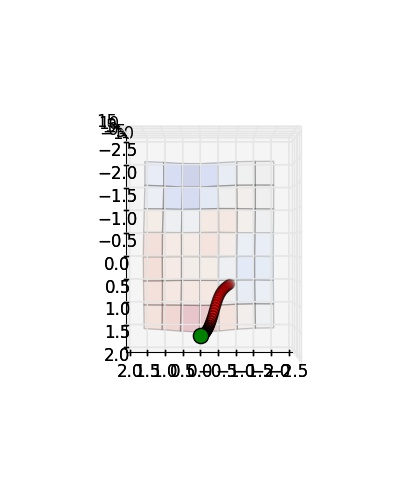
\includegraphics[width=.8\linewidth]{img/ex1/runs/SD-Plateau3D_0_0,07.jpg}
  %was SD-Plateau3D_-0.81  0.59_0.0_0.07
  %\caption{}
  %\label{fig:}
\end{minipage}%
\begin{minipage}{.5\textwidth}
  \centering
  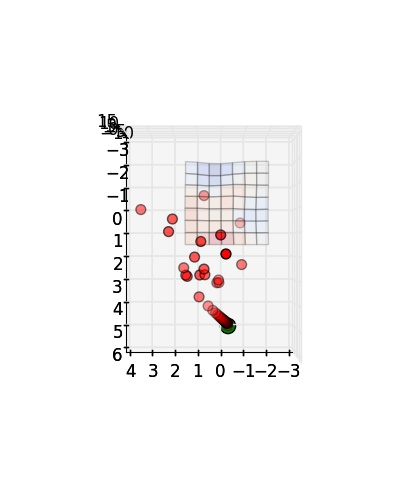
\includegraphics[width=.8\linewidth]{img/ex1/runs/SD-Plateau3D_0,22_0,02.jpg}
  %\caption{}
  %\label{fig:} 
\end{minipage}
\caption{Two highly different runs of the steepest descent algorithm in the Plateau3D landscape. Learning rates of 0.0 (left) and 0.22 (right) and inertia 0.07 (left) and 0.02 (right).}
\label{fig:plateau}
\end{figure}

\subsubsection{Fitness}
Since the algorithms are deterministic for a given set of parameters, it is not necessary to build the mean over a couple of runs. Instead the performance was analysed with respect to to the parameters.\\

\paragraph{Starting position}
The starting position has a huge impact on the performance because it define whether the next optimum is a local or a global one, and how far the algorithm needs to travel. For a 2D landscape the minimum fitness assembles the fitness landscape, while the maximum fitness should point out the optima. As seen in Figure\ref{fig:2dminmax} the optima of the squared error was found independent of the starting position where for the trimodal landscape the Hillclimber (dashed) sometimes could not find a optimum. 
%MEANMAX
\begin{figure}[H]
\centering
\begin{minipage}{.5\textwidth}
  \centering
  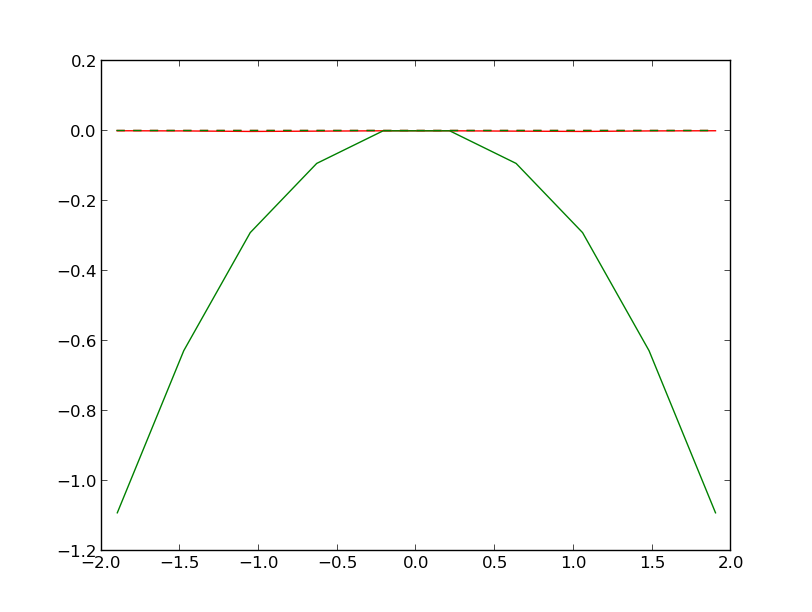
\includegraphics[width=.8\linewidth]{img/ex1/analysis_squared_newton_hill.png}
  %\caption{}
  %\label{fig:}
\end{minipage}%
\begin{minipage}{.5\textwidth}
  \centering
  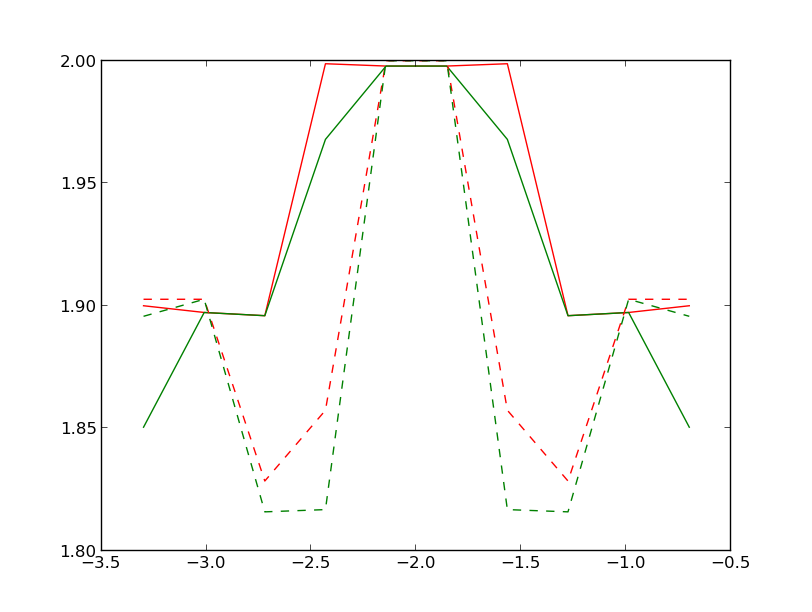
\includegraphics[width=.8\linewidth]{img/ex1/analysis_trimodal_newton_hill.png}
  %\caption{}
  %\label{fig:} 
\end{minipage}
\caption{Fitness analysis of the mean (green) and maximal(red) values of the newton method (solid) and the Hillclimber (dashed).}
\label{fig:2dminmax}
\end{figure}
%Description

In the 3D landscape, the fitness was analysed by a heat map that maps the final fitness to the starting position. All areas of the same color converge to the same fitness. As seen in Figure\ref{fig:heatmap} the Hillclimber often gets stuck at the plateau (blue). With the given parameters, the Hillclimber performed more reliable because it did not overshoot. With the right parameters, the steepest descent did perform better.
 
%HEATMAPS
\begin{figure}[H]
\centering
\begin{minipage}{.5\textwidth}
  \centering
  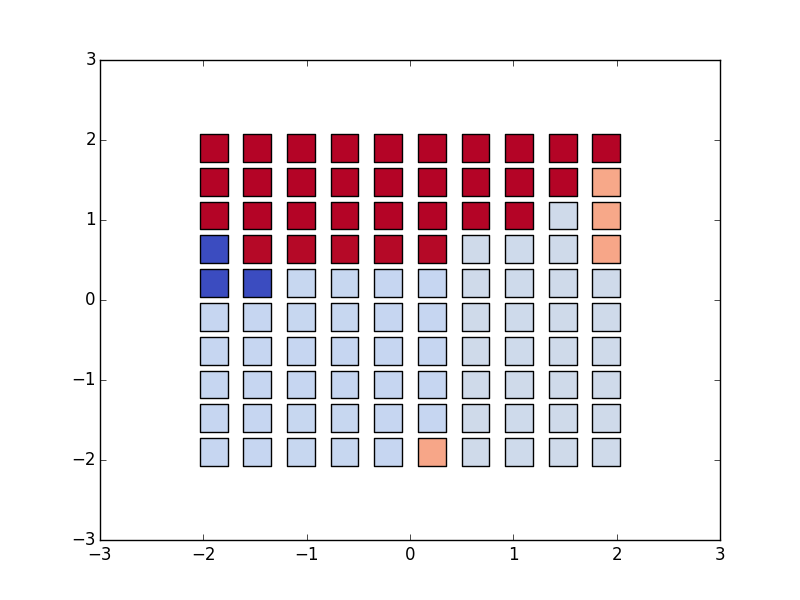
\includegraphics[width=.8\linewidth]{img/ex1/Heatmap_HC.png}
  %\caption{}
  %\label{fig:}
\end{minipage}%
\begin{minipage}{.5\textwidth}
  \centering
  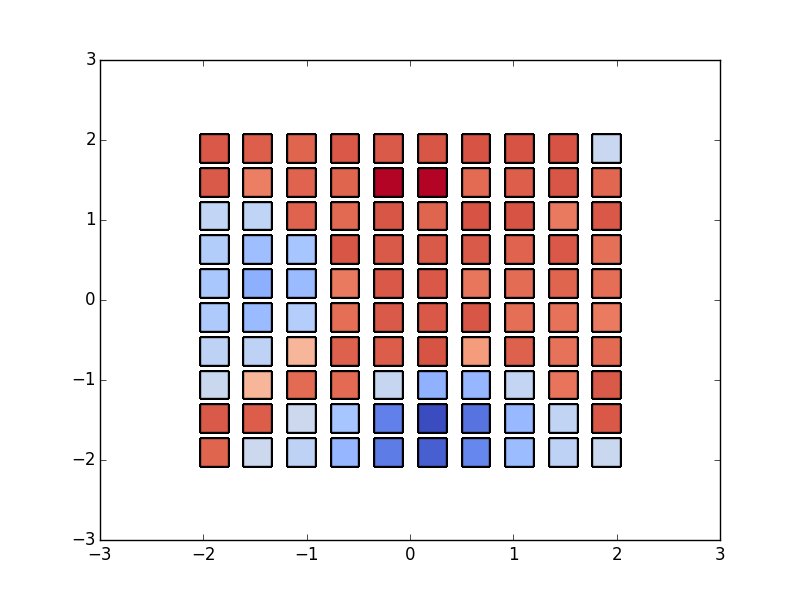
\includegraphics[width=.8\linewidth]{img/ex1/Heatmap_SS.png}
  %\caption{}
  %\label{fig:} 
\end{minipage}
\caption{Heatmap of the fitness values of the Hillclimber (left) and Steepest Descent(right) method in a 3D Landscape.}
\label{fig:heatmap}
\end{figure}

\paragraph{Step width}
The step width is determined by the learning rate and the inertia. Both are crucial to overcome local minima. In Figure \ref{fig:inertialearning} Those parameters are grouped and all final fitness are shown as individual dots. This allows to see how often one parameter reaches an optimal fitness.
As the fitness for the squared error is global by nature and the overshoots in the 3D case, only the trimodal landscape is shown.\\
From the point density one can see that the learning rate(left) is a more reliable way to point towards an optimum while the inertia(right) overcomes the local minima at 1.0 better.

%INERTIA LEARNING
\begin{figure}[H]
\centering
\begin{minipage}{.5\textwidth}
  \centering
  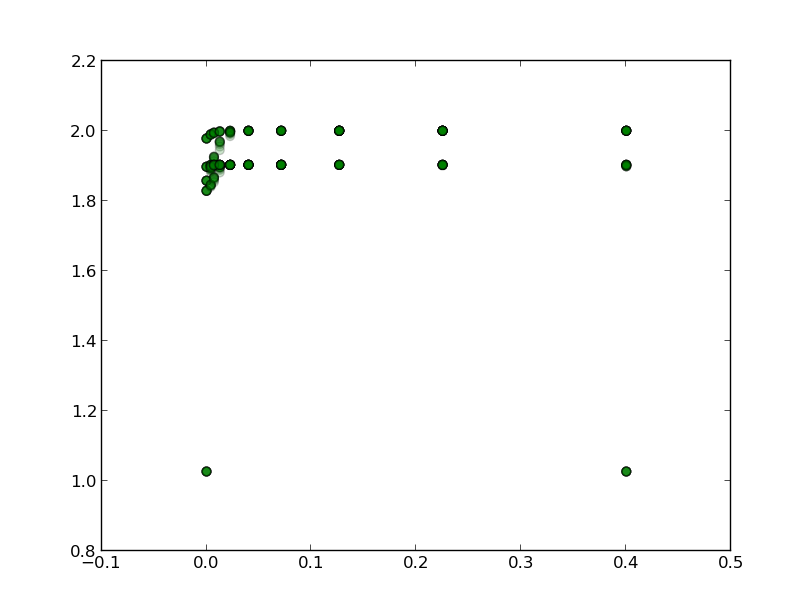
\includegraphics[width=.8\linewidth]{img/ex1/learning_trimodal_ss.png}
  %\caption{}
  %\label{fig:}
\end{minipage}%
\begin{minipage}{.5\textwidth}
  \centering
  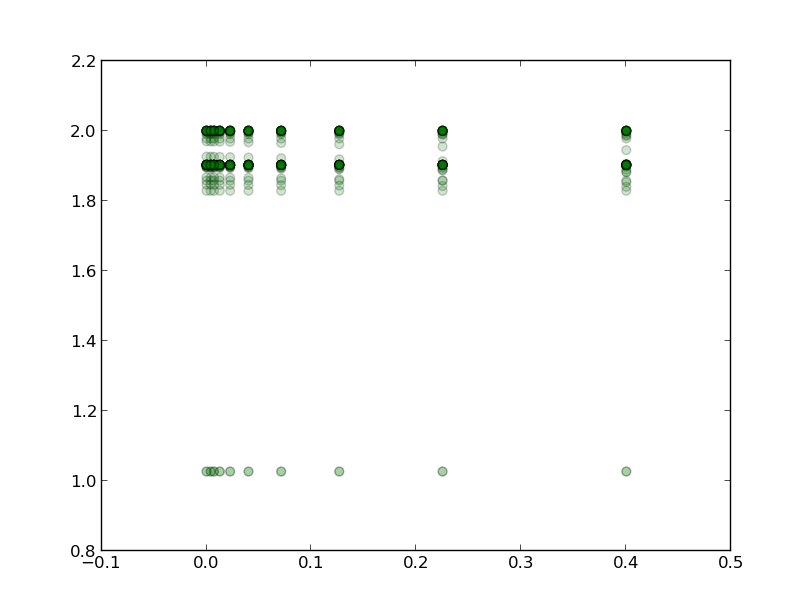
\includegraphics[width=.8\linewidth]{img/ex1/inertia_trimodal_ss.png}
  %\caption{}
  %\label{fig:} 
\end{minipage}
\caption{Comparison of the fitness values with respect to the learning rate (left) and inertia(right) with the steepest descent method on the trimodal landscape.}
\label{fig:inertialearning}
\end{figure}

\subsubsection{Best result}
To discuss the fitness optimality on these landscapes does not give any insight because almost all runs where successfull. However the steps to reach the goals varied, as as shown in Figure \ref{fig:stepssquared}. The Hillclimber took the most steps, while the steepest descents found the optimal quickly. The fastest however has the newtons method.

%RUNS
\begin{figure}[H]
\centering
\begin{minipage}{.5\textwidth}
  \centering
  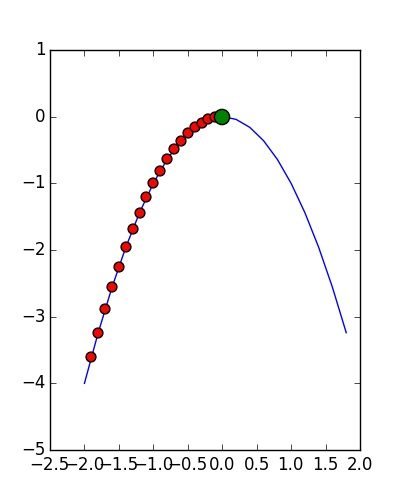
\includegraphics[width=.8\linewidth]{img/ex1/runs/HC-SquaredError2D_-1,9.jpg}
  %\caption{}
  %\label{fig:}
\end{minipage}%
\begin{minipage}{.5\textwidth}
  \centering
  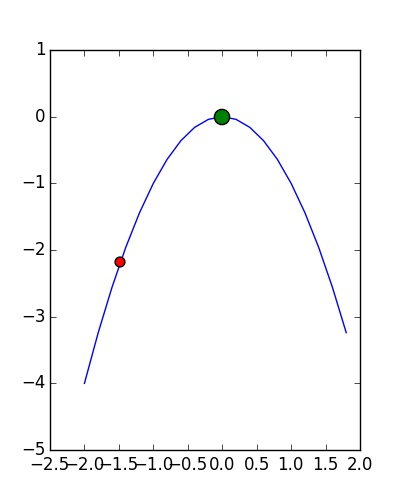
\includegraphics[width=.8\linewidth]{img/ex1/runs/NM-SquaredError2D_-1,48.jpg}
  %\caption{}
  %\label{fig:} 
\end{minipage}
\caption{Incrementing steps of optimization of the Hillclimber (left) and the Newton Method (right) on the squared error landscape.}
\label{fig:stepssquared}
\end{figure}


\subsection{Conclusion}
The varying complexity of the fitness landscape and the degree of information about the landscape used in the algorithms had to match to show a good performance. Thus, the Hillclimber as a mostly uninformed method did a good job on all landscapes but can not overcome local optima. The performance was increased by adapting the step width and direction with a learning rate or the information about the steepest descent. Those however require tuning or additional information. The most complex and effective algorithm, Newtons method performed best.\\
So if we have no additional information about the landscape to optimize, parameter tuning is required. If we have additional information, this can greatly improve the performance. This however is not a likely scenario.



\section{Genetic Algorithms}
%Theoretic description

\subsection{Problem}
%characteristics of the problem

\subsection{Algorithms}
%How do we solve it
real valued, bit string

\subsection{Parameters}
%What could be changed
\subsubsection{Population size}
\subsubsection{Selection}
\subsubsection{Crossover}
\subsubsection{Mutation}


\subsection{Analysis}
%what happened and why

\subsubsection{Parameter variations}

\subsubsection{Fitness}

\subsubsection{Best result}

\subsection{Conclusion}



\section{Travelling Salesman}
%Theoretic description

\subsection{Problem}
%characteristics of the problem
TSP

\subsection{Algorithms}
%How do we solve it

\subsubsection{Representation}
\paragraph{Priority list}
\paragraph{Permutations}

\subsection{Parameters}
%What could be changed
\subsubsection{Population size}

%TSP POP
\begin{figure}
 \center
 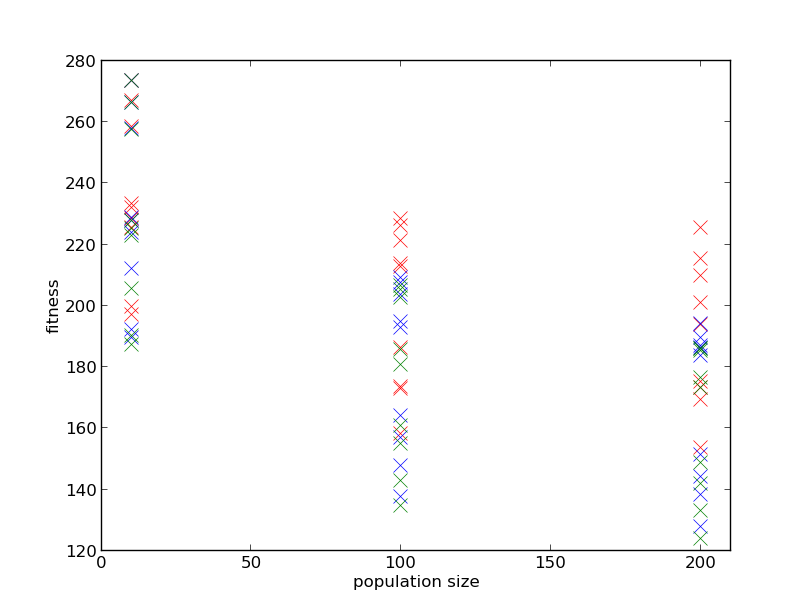
\includegraphics[width=.5\linewidth]{img/ex3/tsp_fitness_population.png}
 \caption{All fitness values (min=green, mean = blue, max = red))ordered by population.}
\end{figure}

\subsubsection{Selection Pressure} 

%TSP Selection
\begin{figure}
 \center
 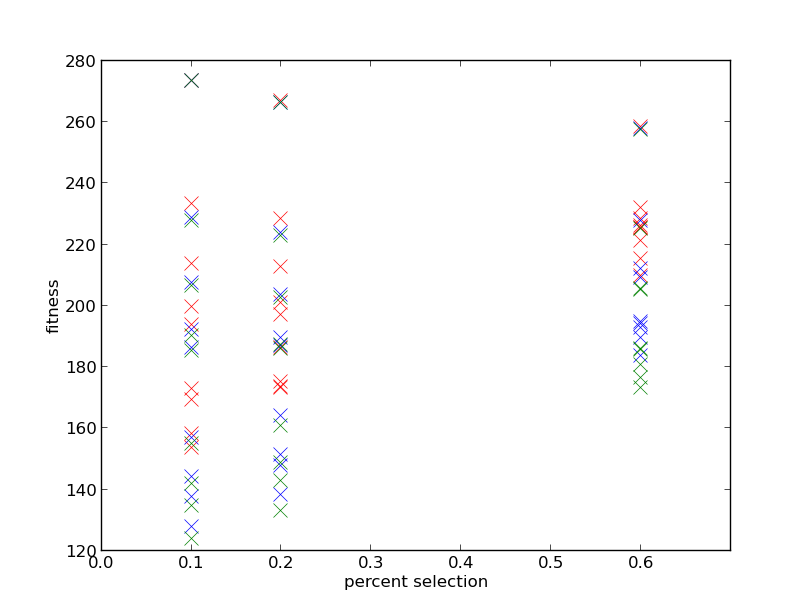
\includegraphics[width=.5\linewidth]{img/ex3/tsp_fitness_selection.png}
 \caption{All fitness values (min=green, mean = blue, max = red))ordered by selection pressure.}
\end{figure}


\subsubsection{Mutation}
%TSP mutations
\begin{figure}
 \center
 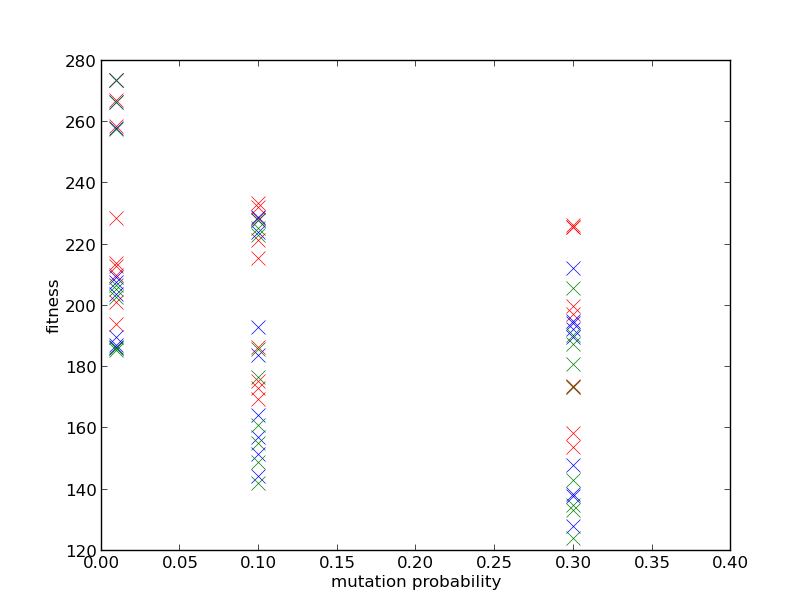
\includegraphics[width=.5\linewidth]{img/ex3/tsp_fitness_mutation.png}
 \caption{All fitness values (min=green, mean = blue, max = red))ordered by selection mutation.}
\end{figure}

\subsection{Analysis}
%what happened and why
Schema Theory
Building Block Hypothesis
Solution Validation

\subsubsection{Fitness}

\subsubsection{Best result}

%TSP BEST
\begin{figure}[H]
\centering
\begin{minipage}{.5\textwidth}
  \centering
  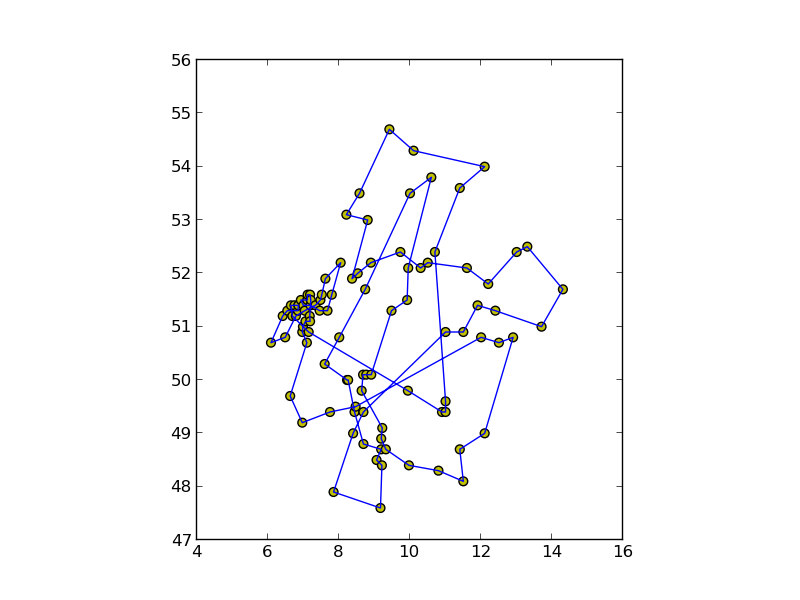
\includegraphics[width=.8\linewidth]{img/ex3/68,46-1-1000-200-0,2-0,6.png}
  %\caption{}
  %\label{fig:}
\end{minipage}%
\begin{minipage}{.5\textwidth}
  \centering
  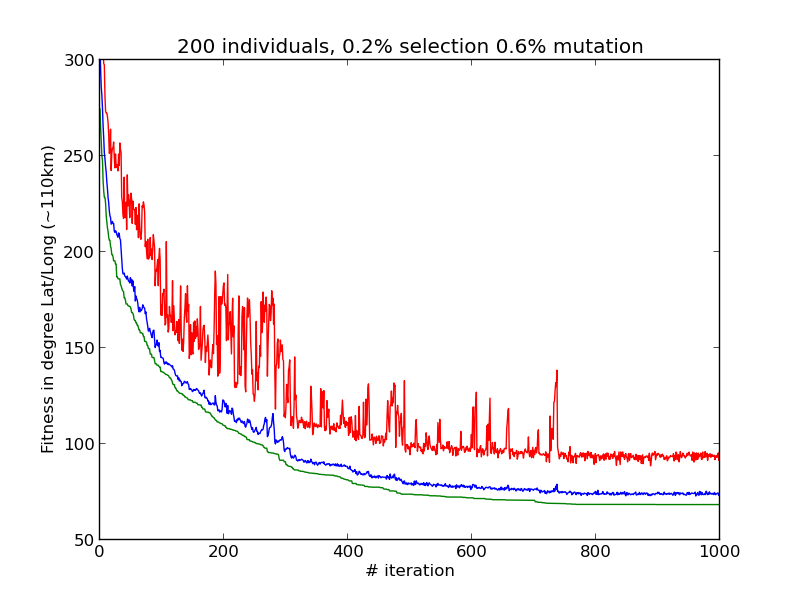
\includegraphics[width=.8\linewidth]{img/ex3/68,46-1-1000-200-0,2-0,6-fitness.png}
  %\caption{}
  %\label{fig:} 
\end{minipage}
\caption{The best run for the travelling salesman. 1k iterations with 200 individuals, a selection of 20\% and mutation rate of 60\% (not 0.2 and 0.6 as in the image). The position of the cities are given in Lat/Long, as well as the fitness. The fitness is given as max(red), mean(blue) and min(green).}
\label{fig:}
\end{figure}
%Description

\subsection{Conclusion}




\section{Evolutionary Algorithm}
%Theoretic description

\subsection{Problem}
%characteristics of the problem

\subsection{Algorithms}
%How do we solve it


\subsection{Parameters}
%What could be changed
\subsubsection{Iterations}
\subsubsection{Sigma/ Sigma Delta}

%SIGMA
\begin{figure}
 \center
 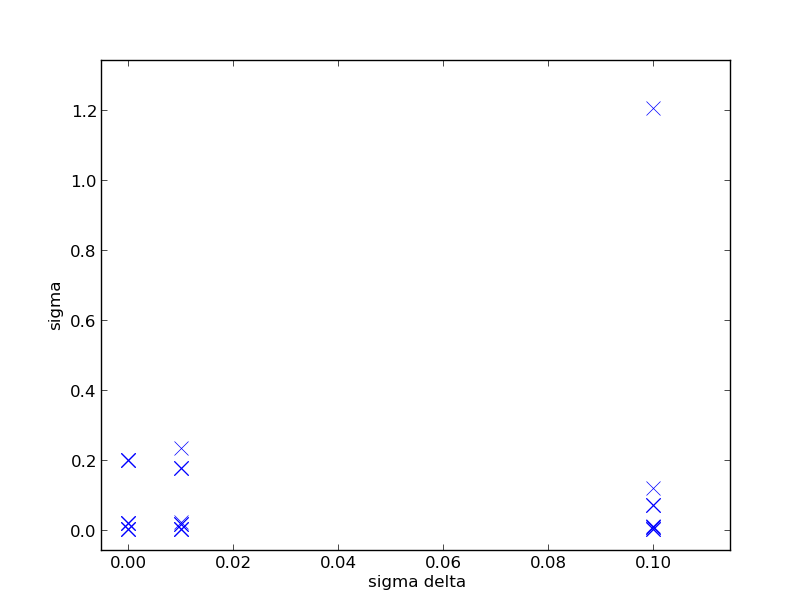
\includegraphics[width=.5\linewidth]{img/ex4/sigmas.png}
 \caption{Final sigma in relation to the sigma delta over all runs.}
\end{figure}

\subsubsection{selection Mode}
\paragraph{$1+1$}

\paragraph{$\mu,\lambda$}

\paragraph{$\mu +\lambda$}


\subsection{Analysis}
%what happened and why


\begin{table}[htbp]
\caption{Fitness over 30 runs each}
\begin{tabular}{r r r|r r }

selection & Sigma $\Delta$ & Sigma & Mean Fitness & Best Fitness \\ \hline
1+1 & 0 & 0.002 & 1228892 & 1228892 \\ 
1+1 & 0.01 & 0.002 & 1228793 & 1228561 \\ 
1+1 & 0.1 & 0.012 & 1225754 & 1221046 \\ 
1+1 & 0 & 0.02 & 1228892 & 1228892 \\ 
1+1 & 0.01 & 0.023 & 1228892 & 1228892 \\ 
1+1 & 0.1 & 0.121 & 1228892 & 1228892 \\ 
1+1 & 0 & 0.2 & 1228892 & 1228892 \\ 
1+1 & 0.01 & 0.234 & 1228892 & 1228892 \\ 
1+1 & 0.1 & 1.206 & 1228892 & 1228892 \\ 
1+20 & 0 & 0.002 & 1224793 & 1220197 \\ 
1+20 & 0.01 & 0.002 & 1220713 & 1213483 \\ 
1+20 & 0.1 & 0.001 & 1225500 & 1222800 \\ 
1+20 & 0 & 0.02 & 1227115 & 1226354 \\ 
1+20 & 0.01 & 0.018 & 1228892 & 1228892 \\ 
1+20 & 0.1 & 0.007 & 1225472 & 1221001 \\ 
1+20 & 0 & 0.2 & \textbf{1188537} & \textbf{1128005} \\ 
1+20 & 0.01 & 0.175 & 1228892 & 1228892 \\ 
1+20 & 0.1 & 0.07 & 1226681 & 1220602 \\ 
2+20 & 0 & 0.002 & 1225606 & 1223490 \\ 
2+20 & 0.01 & 0.002 & 1224471 & 1220651 \\ 
2+20 & 0.1 & 0.001 & 1226304 & 1224964 \\ 
2+20 & 0 & 0.02 & 1228892 & 1228892 \\ 
2+20 & 0.01 & 0.018 & 1227215 & 1221702 \\ 
2+20 & 0.1 & 0.007 & 1211559 & \textbf{1197249} \\ 
2+20 & 0 & 0.2 & 1218575 & \textbf{1190204} \\ 
2+20 & 0.01 & 0.175 & 1228892 & 1228892 \\ 
2+20 & 0.1 & 0.07 & 1228892 & 1228892 \\ 
1,20 & 0 & 0.002 & inf & inf \\ 
\dots & & & \dots & \dots \\
%1,20 & 0.01 & 0.002 & inf & inf \\ 
%1,20 & 0.1 & 0.002 & inf & inf \\ 
%1,20 & 0 & 0.02 & inf & inf \\ 
%1,20 & 0.01 & 0.018 & inf & inf \\ 
%1,20 & 0.1 & 0.007 & inf & inf \\ 
%1,20 & 0 & 0.2 & inf & inf \\ 
%1,20 & 0.01 & 0.175 & inf & inf \\ 
%1,20 & 0.1 & 0.07 & inf & inf \\ 
%2,20 & 0 & 0.002 & inf & inf \\ 
%2,2 & 0.01 & 0.002 & inf & inf \\ 
%2,20 & 0.1 & 0.002 & inf & inf \\ 
%2,20 & 0 & 0.02 & inf & inf \\ 
%2,20 & 0.01 & 0.018 & inf & inf \\ 
%2,20 & 0.1 & 0.007 & inf & inf \\ 
%2,20 & 0 & 0.2 & inf & inf \\ 
%2,20 & 0.01 & 0.175 & inf & inf \\ 
2,20 & 0.1 & 0.07 & inf & inf \\ 
\end{tabular}
\label{}
\end{table}


\subsubsection{Fitness}

\subsubsection{Best result}

%VEHICLE BEST
\begin{figure}
 \center
 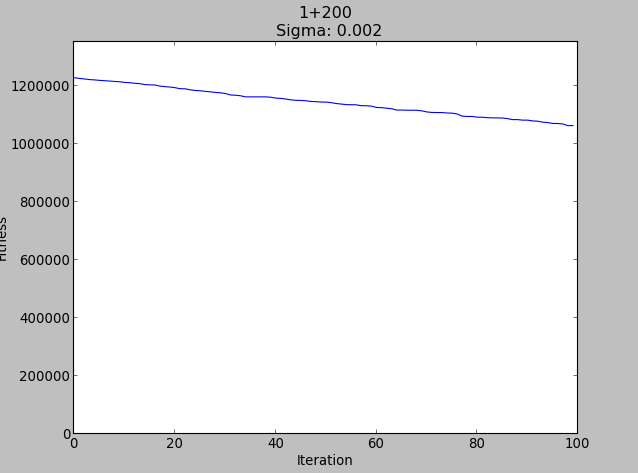
\includegraphics[width=.5\linewidth]{img/ex4/1063459-1+200-0,002.png}
 \caption{Screenshot of the best run with a final fitness of 1063459, and a fixed sigma of 0.002.}
\end{figure}


\subsection{Conclusion}


%CONTENTS
%NOTES


%COPY AND PASTE FROM HERE

%\begin{enumerate}
% \item 
%\end{enumerate}

%\hyperref{link}{text}

%\begin{lstlisting}[language=Python]
%#PYTHON CODE HERE
%\end{lstlisting}

%\lstinputlisting[Language=Python]{ }


%\begin{figure}
% \center
% \includegraphics[width= cm]{ }
% \caption{}
%\end{figure}


%\begin{figure}[H]
%\centering
%\begin{minipage}{.5\textwidth}
%  \centering
%  \includegraphics[width=.8\linewidth]{img/}
%  %\caption{}
%  %\label{fig:}
%\end{minipage}%
%\begin{minipage}{.5\textwidth}
%  \centering
%  \includegraphics[width=.8\linewidth]{img/}
%  %\caption{}
%  %\label{fig:} 
%\end{minipage}
%\caption{}
%\label{fig:}
%\end{figure}
%Description


%BIBLIOGRPAHY?
\bibliographystyle{plain}%amsalpha
\bibliography{Top30.bib}
%\bibentry{}

\end{document}
